\chapter{Ressource: Source-Code} \label{Source-Code}
Der Source-Code ist auf dem beigelegten USB-Stick zu finden.\\
Die Installation von Rasa für das jeweilige Betriebssystem ist auf der Rasa Dokumentationsseite beschrieben: 
\url{https://rasa.com/docs/rasa/installation/}.

Für die Ausführung des beigelegten Quellcodes müssen folgende Terminal Befehle (im Source-Code Directory) erfolgen:
\begin{itemize}
  \item pip install fuzzywuzzy
  \item install xlwt
  \item install xlrd 
  \item pip install sanic==21.9.3
\end{itemize}

Anschließend sollten zwei Terminal Fenster geöffnet werden. In beiden Terminals wird zum Ordner navigiert, der den Source-Code enthält.
Sofern noch kein Model vorliegt, muss zuerst der Befehl \textit{rasa train} folgen. Anschließend bedarf es an folgenden Befehlen:
\begin{itemize}
  \item \textbf{Terminal 1:} \\
        rasa shell
  \item \textbf{Terminal 2:} \\
        rasa run actions
\end{itemize}

Sofern die Rasa X UI gewünscht ist, benötigt es an folgendem Installationsbefehl:\\
pip install rasa-x --extra-index-url https://pypi.rasa.com/simple \\ 
Anschließend folgt in Terminal 1 an der Stelle von rasa shell \textit{rasa x}.

Sollte es beim Aufruf von Rasa Probleme geben, wie z.B. \glqq rasa command not found\grqq{}, muss der Path von Python exportiert werden.
Folgender Befehl im Terminal (in dem Source-Code Directory) ist vor den Rasa Anweisungen (rasa shell oder rasa x \& rasa run actions) nötig:\\
export PATH=\$PATH:/Users/username/Library/Python/3.8/bin


\chapter{Ressource: ILS-Fragebogen} 

Es werden zuerst die ausgewählten 17 reduzierten ILS-Fragen aufgeführt. Anschließend folgt der vollständige ILS-Fragebogen

\section{17-ILS-Fragebogen} \label{17-ILS-Fragebogen}

\begingroup
  \footnotesize  
\begin{longtable}{|m{1cm}|m{7.75cm}|m{3.0cm}|m{2.4cm}|}
  \hline
\rowcolor[HTML]{EFEFEF} 
\centering \textbf{Index} & \centering \textbf{ILS-Frage}& \centering \textbf{ILS-Index \&} \textbf{FS-Dimension}& \centering \arraybackslash \textbf{Kategorie} \\ 
\hline \hline 
Q1 & \begin{tabular}[c]{@{}l@{}}When I think about what I did yesterday, \\ I am most likely to remember  \\  (a) a picture. \\  (b) words.\end{tabular} & \begin{tabular}[c]{@{}l@{}} (Q3) \\ visuell/verbal \end{tabular} & \multicolumn{1}{c|}{} \\ \cline{1-3}
Q2 & \begin{tabular}[c]{@{}l@{}}When I get directions to a new place, I prefer \\ (a) a map.\\ (b) written instructions.\end{tabular} & \begin{tabular}[c]{@{}l@{}} (Q23) \\ visuell/verbal  \end{tabular}&  {\textbf{Smalltalk}}\\ \cline{1-3}
Q3 & \begin{tabular}[c]{@{}l@{}}When someone is showing me data, I prefer \\ (a) charts or graphs. \\ (b) text summarizing the results.\end{tabular} & \begin{tabular}[c]{@{}l@{}} (Q31) \\ visuell/verbal  \end{tabular}&  \\ \hline
Q4 & \begin{tabular}[c]{@{}l@{}}I would rather first \\  (a) try things out,\\  (b) think about how I'm going to do it.\end{tabular} & \begin{tabular}[c]{@{}l@{}} (Q25) \\ aktiv/reflektiv  \end{tabular}&  \\ \cline{1-3}
Q5 & \begin{tabular}[c]{@{}l@{}}I would rather be considered \\  (a) realistic. \\  (b) innovative.\end{tabular} & \begin{tabular}[c]{@{}l@{}} (Q2) \\ sensorisch/intuitiv  \end{tabular}& {\textbf{Persönlichkeit}} \\ \cline{1-3}
Q6 & \begin{tabular}[c]{@{}l@{}}I prefer the idea of\\ (a) certainty.\\ (b) theory.\end{tabular} & \begin{tabular}[c]{@{}l@{}}  (Q18) \\ sensorisch/intuitiv  \end{tabular}&   \\ \hline
Q7 & \begin{tabular}[c]{@{}l@{}}When I start a homework problem, \\ I am more likely to\\ (a) start working on the solution immediately. \\ (b) try to fully understand the problem first.\end{tabular} & \begin{tabular}[c]{@{}l@{}} (Q17) \\ aktiv/reflektiv  \end{tabular}&  \\ \cline{1-3}
Q8 & \begin{tabular}[c]{@{}l@{}}I prefer courses that emphasise \\ (a) concrete material (facts, data). \\ (b) abstract material (concepts, theories).\end{tabular} & \begin{tabular}[c]{@{}l@{}} (Q38) \\ sensorisch/intuitiv  \end{tabular}&  \\ \cline{1-3}
Q9 & \begin{tabular}[c]{@{}l@{}}I find it easier \\ (a) to learn facts.\\ (b) to learn concepts.\end{tabular} & \begin{tabular}[c]{@{}l@{}} (Q10) \\ sensorisch/intuitiv  \end{tabular}&  \\ \cline{1-3}
Q10 & \begin{tabular}[c]{@{}l@{}}I learn \\ (a) at a fairly regular pace. If I study hard,\\ I'll get it.\\ (b) in fits and starts. I'll be totally confused\\ and then suddenly it all "clicks."\end{tabular} & \begin{tabular}[c]{@{}l@{}} (Q24) \\ sequentiell/global  \end{tabular}&  \\ \cline{1-3}
Q11 & \begin{tabular}[c]{@{}l@{}}When I am learning a new subject, I prefer to \\ (a) stay focused on that subject,\\ learning as much about it as I can. \\ (b) try to make connections between that subject\\ and related subjects.\end{tabular} &\begin{tabular}[c]{@{}l@{}}  (Q36) \\ sequentiell/global  \end{tabular}&  {\textbf{Studienleben}}\\ \cline{1-3}
Q12 & \begin{tabular}[c]{@{}l@{}}I prefer to get new information in \\ (a) pictures, diagrams, graphs, or maps. \\ (b) written directions or verbal information.\end{tabular} & \begin{tabular}[c]{@{}l@{}} (Q7) \\ visuell/verbal  \end{tabular} &  \\ \cline{1-3}
Q13 & \begin{tabular}[c]{@{}l@{}}In a book with lots of pictures and charts,\\  I am likely to\\ (a) look over the pictures and charts carefully.\\ (b) focus on the written text.\end{tabular} & \begin{tabular}[c]{@{}l@{}} (Q11) \\ visuell/verbal  \end{tabular} &  \\ \cline{1-3}
Q14 & \begin{tabular}[c]{@{}l@{}}When I see a diagram or sketch in class, \\ I am most likely to remember          \\ (a) the picture. \\ (b) what the instructor said about it.\end{tabular} & \begin{tabular}[c]{@{}l@{}} (Q27) \\ visuell/verbal  \end{tabular} &  \\ \cline{1-3}
Q15 & \begin{tabular}[c]{@{}l@{}}When solving problems in a group,\\ I would be more likely to \\ (a) think of the steps in the solution process. \\ (b) think of possible consequences\\ or applications of the solution in a wide range \\ of areas.\end{tabular} & \begin{tabular}[c]{@{}l@{}} (Q44) \\ sequentiell/global  \end{tabular}&  \\ \cline{1-3}
Q16 & \begin{tabular}[c]{@{}l@{}}I am more likely to be considered \\ (a) careful about the details of my work. \\ (b) creative about how to do my work.\end{tabular} & \begin{tabular}[c]{@{}l@{}} (Q22) \\ sensorisch/intuitiv  \end{tabular}&  \\ \cline{1-3}
Q17 & \begin{tabular}[c]{@{}l@{}}If I were a teacher, I would rather teach a course \\ (a) that deals with facts and real life situations.\\ (b) that deals with ideas and theories.\end{tabular} & \begin{tabular}[c]{@{}l@{}} (Q6) \\ sensorisch/intuitiv  \end{tabular}&  \\ \hline 
\caption[Kategorisierung der ILS-Fragen]{Kategorisierung der ILS-Fragen in Anlehnung an \parencite[51 f.]{Latham.2011}} 
\label{tab:/Kategorisierung der ILS-Fragen} 
\end{longtable}
\endgroup

\section{44-ILS-Fragebogen}

Auf den nachfolgenden Seiten befindet sich der vollständige ILS-Fragebogen. \parencite{ILS.1991}  \label{44ILS}

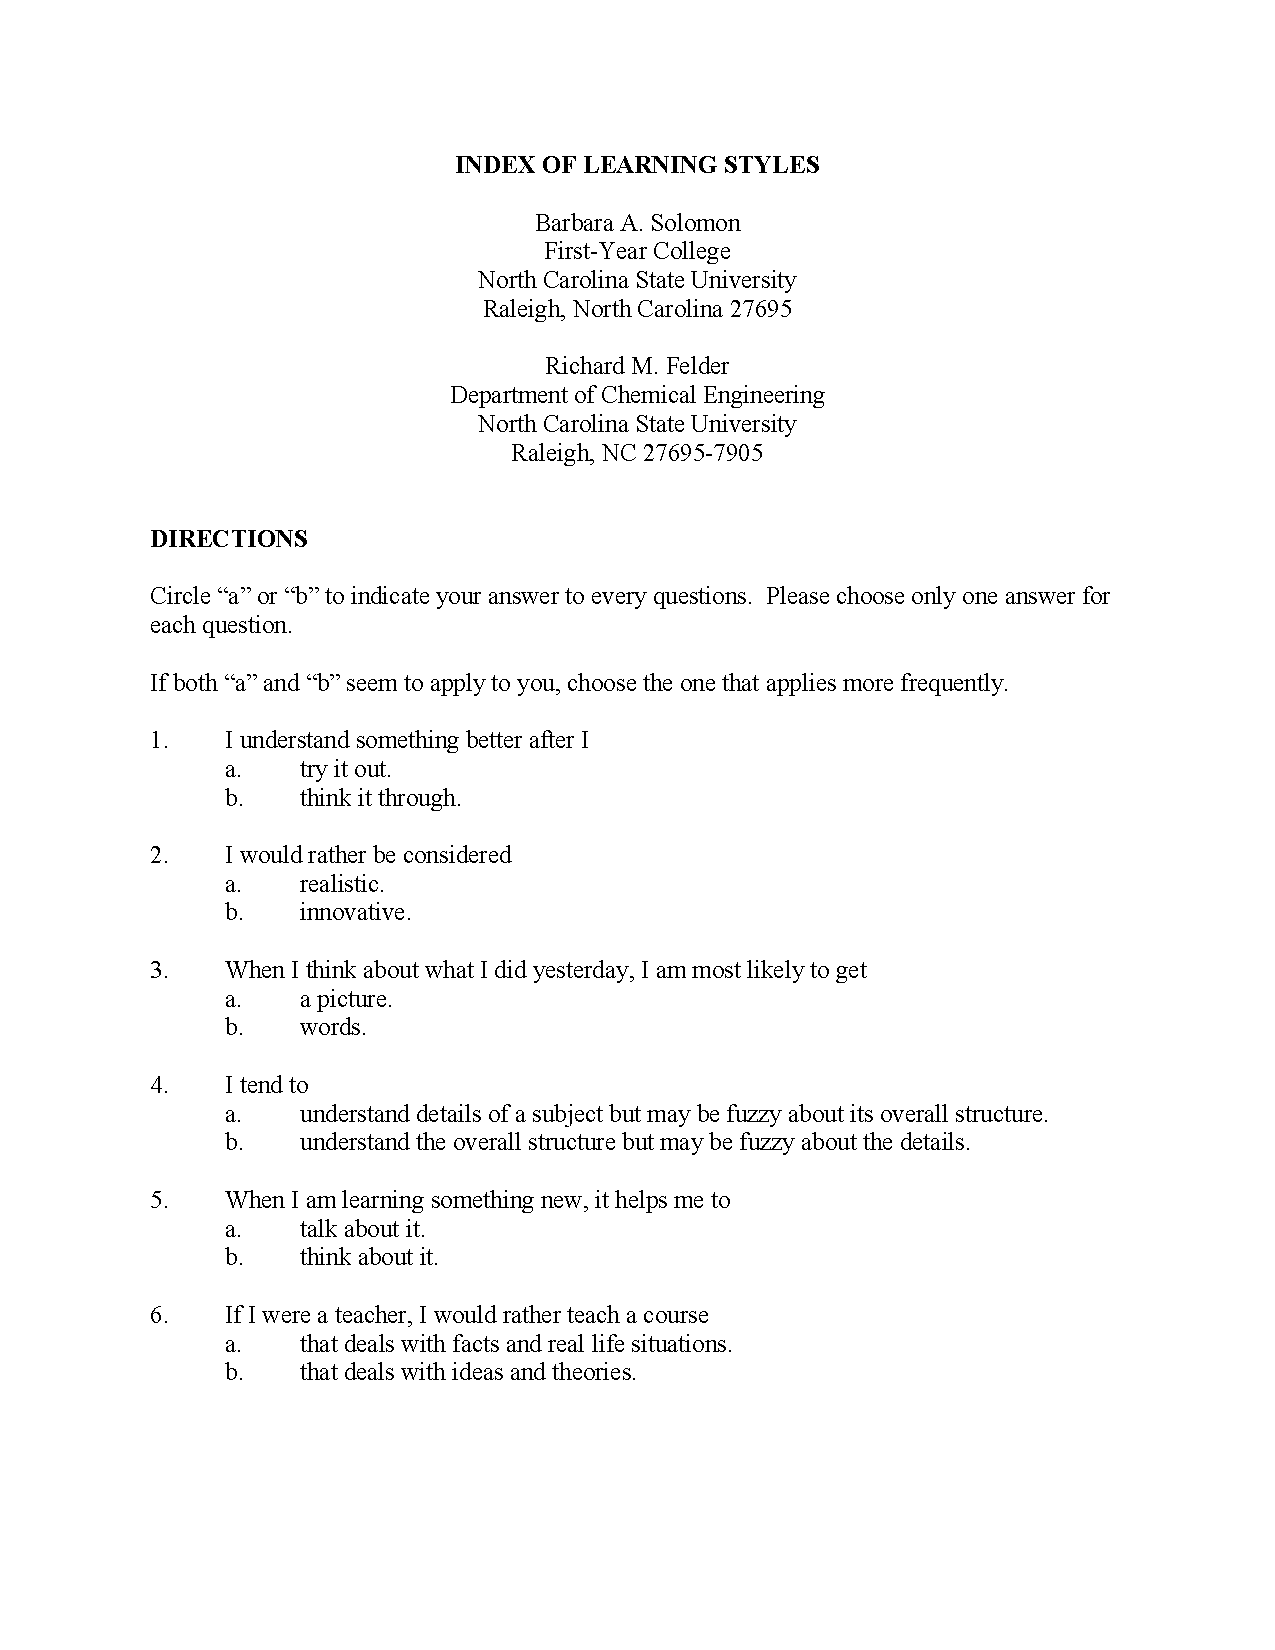
\includepdf[pages=-]{Fragebogen/ILS.pdf}


\chapter{Dialog}
\section{Wizard of OZ}   \label{tab:/Anhang_Dialogflow/G} 

\begingroup
  \footnotesize  
\begin{longtable}{|m{2.5cm}|m{12.0cm}|}
  \hline     
  \rowcolor[HTML]{EFEFEF}                                         
  \textbf{Teilnehmer} & \textbf{Gesprächsdialog: Greeting } \\ 
  \hline \hline  
  Prototyp: & Hey mate! I´m Vicky nice to meet you. What´s your name ?    \\ \hline
  Testperson: & Hey Vicky! I´ m Lotta\\ \hline
  \hline    
  Prototyp: & Hey Lotta, How are you?  \\  \hline  
  Testperson: & I ´m fine, thanks and you?\\ \hline
  \hline   
  Prototyp: & I´m good too thanks.  \\  \hline  
\end{longtable}
\endgroup  

\begingroup
  \footnotesize 
\begin{longtable}{|m{2.5cm}|m{12.0cm}|}
  \hline     
  \rowcolor[HTML]{EFEFEF}                                         
  \textbf{Teilnehmer} & \textbf{Gesprächsdialog: Smalltalk } \\ 
  \hline \hline  
  
  Prototyp: & I would like to get you better known. What did you do yesterday in the evening?  \\  \hline  
  Testperson: & I‘ve been doing some sport with my boyfriend and later wie ate dinner together and watched our  series…\\ \hline
  \hline 

  Prototyp: & Nice. When you thought about what you did yesterday in the evening. Did you memorize it like to get a picture or words? \\  \hline  
  Testperson: & I guess for me is more like a picture than a text.\\ \hline
   

  Frage/FS-Dimension: & Q3 visual/verbal \\ \hline
  \hline 

  Prototyp: & Okay got it. I´m a litte bit shocked about the actual situation because of Covid. Therefore 
               it´s a little bit difficult to travel around at the moment. But imagine if you get to a new place 
          would you prefer a map or a written instruction?\\  \hline  
  Testperson: & Oh yes I feel that too… I think I would prefer to see it on a map, for me that is much easier to remember. \\ \hline
   

  Frage/FS-Dimension: & Q23 visual/verbal \\ \hline
  \hline 

  Prototyp: & So if I would give you the newest corona data. 
         Would you like to get them as a chart/ graph diagram
         or as a text summarization\\  \hline  
  Testperson: & I would like to see it as a diagram or something like that. \\ \hline
   

  Frage/FS-Dimension: & Q31 visual/verbal \\ \hline
  \hline 

  Prototyp: & Okay. But I think we should waste so much time with the pandemic. \\ \hline
\end{longtable}
\endgroup  


\begingroup
  \footnotesize 
\begin{longtable}{|m{2.5cm}|m{12.0cm}|}
  \hline     
  \rowcolor[HTML]{EFEFEF}                                         
  \textbf{Teilnehmer} & \textbf{Gesprächsdialog: Persönlichkeit } \\ 
  \hline \hline  
  
  Prototyp: &  I´m interested in your personality.
  So if you get known to a new thing. Would you first try them out or think about how you are going to do it. \\  \hline  
Testperson: & I think it depends on what we are talking about, sometimes I would just try but in other situations
I would like to know at least a little bit what I am about to do… \\ \hline
 

Frage/FS-Dimension: & Q25 active/reflective \\ \hline
\hline 

Prototyp: & I understand. Would you rather be considered realistic or innovative?  \\  \hline  
Testperson: & I think if I am honest I am more a realistic person, but don‘t you think most of the people would like to be innovative? \\ \hline
 

Frage/FS-Dimension: & Q2 sensory/intuitve \\ \hline
\hline 

Prototyp: & And do you like the idea of certainty or theory?  \\  \hline  
Testperson: & think if I like the idea of certainty.  \\ \hline
 

Frage/FS-Dimension: & Q18 sensory/intuitve \\ \hline
\end{longtable}
\endgroup  

\begingroup
  \footnotesize 
\begin{longtable}{|m{2.5cm}|m{12.0cm}|}
  \hline     
  \rowcolor[HTML]{EFEFEF}                                         
  \textbf{Teilnehmer} & \textbf{Gesprächsdialog: Studienleben } \\ 
  \hline \hline  
  Prototyp: & You are a quite cool person. It´s a pleasure to get you known. Let´s talk about your studylife.
  If you get a exercise problem or you have to prepare a presentation or something like this. 
  Do you start working on the solution immediately 
  or do you try to fully understand the problem first?\\  \hline  
  Testperson: & I would start to work on the problem immediately and try to understand the whole thing while working on it.  
            I think it‘s because I think that would be faster…\\ \hline
             

  Frage/FS-Dimension: & Q17 active/reflective \\ \hline
\hline 

Prototyp: & Of course. How are your courses? Do you prefer courses that emphasize concrete material like facts and data or abstract material like 
            concepts, theories\\  \hline  
Testperson: & I am more interested in  concrete material like facts an data.  \\ \hline
Frage/FS-Dimension: & Q38 sensory/intuitive \\ \hline 
\hline

Prototyp: & For me again please. So do you find it easier to learn facts or to learn concepts?\\  \hline  
Testperson: &Yes I find it easier to learn facts than to learn concepts. \\ \hline
 

Frage/FS-Dimension: & Q10 sensory/intuitive \\ \hline   
\hline

Prototyp: & Ah okay, I understand. Are you a person who learns at a fairly regular pace. I mean if you study hard you´ll get it.
Or are you totally confused at the beginning and suddenly all clicks.  \\  \hline  
Testperson: & I think for me it is more like you described first. If I‘m working a lot on something I get it step by step. I guess with learning facts that is the way you have to go… \\ \hline
 

Frage/FS-Dimension: & Q24 sequential/global \\ \hline   
\hline

Prototyp: & And when you are learning a new subject do you prefer to stay focused on that subject and learning as much as you can. Or 
          do you try to make connections between that subject and related subjects?   \\  \hline  
Testperson: & I think for me I prefer to stay focused on the subject. \\ \hline
 

Frage/FS-Dimension: & Q36 sequential/global \\ \hline   
\hline

Prototyp: & Okay. Do you prefer to get new information in pictures, graphs and diagrams or as written, verbal information   \\  \hline  
Testperson: &Pictures, graphs \\ \hline
 

Frage/FS-Dimension: & Q7 visual/verbal \\ \hline   
\hline

Prototyp: & That means if you look in a book with lots of pictures and charts. Do you likely look over the pictures and diagrams 
carefully or do you focus on the wirtten text? \\  \hline  
Testperson: & For me it is easier to understand it by looking at the pictures and charts,
 but sometimes it is helpful to read the text for a better understanding of the pictures and charts.\\ \hline
  

 Frage/FS-Dimension: & Q11 visual/verbal \\ \hline   
\hline

Prototyp: & Does it mean when you see a diagram or sketch in class do you likely to remember the picture or that what the 
        instructor said about it?\\  \hline  
Testperson: & the picture\\ \hline
 

Frage/FS-Dimension: & Q27 visual/ Verbal \\ \hline   
\hline

Prototyp: & Nice. When you solving Problems do you prefer to do it step by step or do you think of possible consequences 
              of the solution in a wide range of areas ?\\  \hline  
Testperson: &I do it step by step \\ \hline
 

Frage/FS-Dimension: & Q44 sequential/global \\ \hline   
\hline

Prototyp: &One thing that would be interesting for me is are you more likely to be considered
            careful about the details of your work or creative about how to do your work? \\ \hline  
Testperson: & I am more careful about the details\\ \hline
 

Frage/FS-Dimension: & Q22 sensory/intuitiv \\ \hline   
\hline

Prototyp: &Imagine you were a teacher, would you rather teach a course that deals with facts and real life situations
          or that deals with ideas and theories? \\ \hline
Testperson: & I´d prefer a course dealing with facts and real life situations\\ \hline
  

Frage/FS-Dimension: & Q6 sensory/ intuitiv \\ \hline   
\hline

Prototyp: & Do you wanna become a teacher ? Or What kind of job would you like to do ?\\ \hline
Testperson: & I am  studying medicine, so I would like to become a doctor, but I‘ve been thinking about becoming a teacher when I was younger.\\ \hline
\end{longtable}
\endgroup  


\section{Synonyme} \label{SynonymeAnhang}

\begin{longtable}{|m{4cm}|m{4.0cm}|m{4.0cm}|}
  \hline   
  \rowcolor[HTML]{EFEFEF} 
  \centering text summarization & \centering visual & \centering \arraybackslash verbal \\ \hline  
  sum up & visible, movie, image & speech, conversation \\\hline  \hline  
  
  \rowcolor[HTML]{EFEFEF} 
  \centering sketch & \centering instructor &\centering \arraybackslash  try\\ \hline  
  draft, drawing &  teacher, supervisor & attemp, undertake \\\hline  \hline  
  
  \rowcolor[HTML]{EFEFEF} 
  \centering plan & \centering start &\centering \arraybackslash  understand\\ \hline  
   preperation &  begin, take up & appreciate, recognize, realize  \\\hline  \hline
   
   \rowcolor[HTML]{EFEFEF} 
   \centering realistic & \centering concrete & \centering \arraybackslash  abstract\\ \hline  
   practical, pragmatic  &  factual, existing, pyhsical & theoretical \\\hline  \hline  

   \rowcolor[HTML]{EFEFEF} 
   \centering speed & \centering step &   \centering \arraybackslash connections\\ \hline  
   tempo  & slowly & relations, association, links  \\\hline  \hline  

   \rowcolor[HTML]{EFEFEF}
   \centering stay focus & \centering certainty &   \centering \arraybackslash carful\\\hline
   stay on, keep on & truth & attentive, wary\\\hline  \hline 

   \rowcolor[HTML]{EFEFEF}  
   \centering creative &   \centering \arraybackslash regular & \\ \hline 
   imaginative, inspired & efficient, structured   &\\ \hline  
  \end{longtable}



\chapter{Quiz-Spiel} 

\section{Lernverhaltensmerkmale}

\begingroup \label{Prototyp_Anhang}
  \footnotesize 
\begin{longtable}{|m{7.5cm}|m{7.5cm}|}
  \hline     
  \rowcolor[HTML]{EFEFEF}                                         
  \centering \textbf{Lernverhalten beim Lernstil} & \centering \arraybackslash \textbf{Folgerung auf den Lernstil} \\ 
  \hline  \hline 
   

  \multicolumn{2}{|c|}{\textbf{sensorisch}} \\ \hline \hline 
  Bevorzugen Fakten, Daten, Experimente & Besseres Abschneiden bei Fragen mit Fakten und Beispielen  \\ \hline
  Abneigung gegen Überraschungen & Bevorzugen Einführungen in das Thema, Übersichten und die Arbeit in einer sequentiellen vorhersehbaren Reihenfolge \\ \hline
  Sorgfältig, aber langsam & Berücksichtigung der Anzahl der Flüchtigkeitsfehler \\ \hline
  Vertraut mit Symbolen (z.B. Wörtern) & Umfang der Diskussion mit dem Tutor berücksichtigen\\ \hline  \hline   
   

  \multicolumn{2}{|c|}{\textbf{intuitiv}} \\ \hline \hline 
  Bevorzugen Prinzipien und Theorien & Besseres Abschneiden bei theoretischen Fragen \\ \hline
  Gelangweilt bei Details & Bessere Leistung, wenn die Informationen zusammengefasst werden \\ \hline
  Schnell, aber unvorsichtig & Berücksichtigung der Anzahl der Flüchtigkeitsfehler \\ \hline
  Nicht vertraut mit Symbolen & Umfang der Diskussion mit dem Tutor berücksichtigen \\ \hline  \hline 
   
  
  \multicolumn{2}{|c|}{\textbf{visuell}} \\ \hline \hline 
  Erinnern sich an das, was sie sehen & Besseres Abschneiden bei Fragen mit Diagrammen und Bildern, Filmen \\ \hline
  Bevorzugen Bilder und Diagramme & Besseres Abschneiden bei Fragen mit Bildern und Diagrammen \\ \hline
  Bevorzugen visuelle Präsentationen & Besseres Abschneiden bei Fragen mit visuellen Erklärungen \\ \hline  \hline   
   

  \multicolumn{2}{|c|}{\textbf{verbal}} \\ \hline \hline 
  Erinnern sich an das, was sie hören, oder was sie hören und dann sagen & Besseres Abschneiden bei Fragen mit Filmen und Soundclips \\ \hline
  Bevorzugen mündliche Erklärung  & Erklärungen des Tutors\\ \hline  \hline   
   

  \multicolumn{2}{|c|}{\textbf{aktiv}} \\ \hline \hline 
  Informationen verarbeiten, indem sie ein Experiment durchführen & Bessere Leistungen bei Fragen mit praktischen Übungen \\ \hline  \hline   
   

  \multicolumn{2}{|c|}{\textbf{reflektiv}} \\ \hline \hline 
  Informationen prüfen und selbständig bearbeiten (Theoretiker) & Bessere Leistungen bei theoretischen Fragen \\ \hline  \hline   
   

  \multicolumn{2}{|c|}{\textbf{sequentiell}} \\ \hline \hline 
  Verfolgen einen linearen Denkprozess, Informationen sollten in einer stetigen Progression von Komplexität gegeben werden &
  Bessere Leistung, wenn die Informationen in einem stetigen Grad von Komplexität ansteigen \\ \hline \hline   
   

  \multicolumn{2}{|c|}{\textbf{global}} \\ \hline \hline 
  Springen direkt zu komplexerem und schwierigem Material &
  Sie sind besser, wenn die Informationen zusammengefasst sind, und wenn sie die Aufgaben in einem Durchgang lösen können. \\ \hline
\caption[Lernverhaltensmerkmale und Lernstil]{Lernverhaltensmerkmale und Lernstil  (eigene Darstellung, in Anlehnung an \parencite[56]{Latham.2011}) } 
\label{tab:/Lernverhaltensmerkmale_Anhang} 
\end{longtable}
\endgroup

\section{Logische Regeln}\label{LogicRulesAnhang}

\begingroup
  \footnotesize  
\begin{enumerate}  
  \item Textbeschreibung:\\
  IF(answer IS(wrong OR don´t know) AND give-theory-explanation)\\
  THEN \\
  IF(next-answer = right)\\
  THEN\\
  (INCREMENT INTUITOR);
  \item Videohilfe:\\
  IF(answer IS(wrong OR don´t know) AND show-movie)\\
  THEN\\
  IF(next-answer = right)\\
  THEN\\
  (INCREMENT VISUAL) AND (INCREMENT VERBAL);
  \item Bildhilfe:\\
  IF(answer IS(wrong OR don´t know) AND show-image)\\
  THEN\\
  IF(next-answer = right)\\
  THEN\\
  (INCREMENT VISUAL);
  \item Beispielhilfe:\\
  IF(answer IS(wrong OR don´t know) AND show-example)\\
  THEN\\
  IF(next-answer = right)\\
  THEN\\
  (INCREMENT SENSOR);
  \item Kleiner Fehler:\\
  IF(mostly correct AND small-mistakes)\\
  THEN\\
  (INCREMENT INTUITOR);
  \item Richtige Antwort nach dem ersten Versuch:\\
  IF(answer = right AND attemp = 1)\\
  THEN\\
  (INCREMENT INTUITOR) AND (INCREMENT GLOBAL);
  \item Lösung ohne Hilfe: \\ \label{RulesI}
  IF(student choose onego)\\
  THEN 
  (INCREMENT GLOBAL) AND  (INCREMENT INTUITOR);
  \item Schrittweise zur Lösung: \\
  IF(student choose steps or don´t know)\\
  THEN 
  (INCREMENT SEQUENTIAL) AND  (INCREMENT REFLECTIVE);
  \item Schrittweise mit Hilfe oder Lösung ohne Hilfe : \\
  IF((student choose steps or onego) AND (wrong answer > 1 OR don´t know > 1))\\
  THEN 
  (INCREMENT SEQUENTIAL) AND  (INCREMENT VERBAL);
  \item Trickfrage: \\ \label{RulesII}
  IF(student answer correct first time without help)\\
  THEN 
  (INCREMENT SENSOR) AND  (INCREMENT VERBAL);\\
  ELSE\\ 
  (INCREMENT INTUITOR) AND (INCREMENT VISUAL);
  \item Fragetyp:\\
  IF(answer is right)\\
  THEN \\
  IF(question type IS practical)\\
  THEN\\
  (INCREMENT ACTIVE) AND (INCREMENT SENSOR)\\
  ELSE IF(question type IS theoretical)\\
  THEN\\
  (INCREMENT REFLECTIVE) AND (INCREMENT INTUITOR)
\end{enumerate}
\endgroup 

\section{Quiz-Spiel-Fragen} \label{FragenQuizSpiel}

Folgende Fragen wurden ausgewählt:
\begin{enumerate}
  \item What day follows the day before yesterday if two days from now (now is fictional and might not be the actual day) will be Sunday? (in Anlehnung an \parencite[6]{Gruber.2010})
  \item Is the left or the right fraction greater or are both equal: 5/19 or 3/29 ? (in Anlehnung an \parencite[30]{Gruber.2010})
  \item What is the next number in the following sequence: 0 0 I III III VI V IX VII XII IX ? (in Anlehnung an \parencite[7]{Gruber.2010})
  \item What is the relationship between the greenhouse effect and sunlight? \footnote{\url{https://assets.pearsonschool.com/asset_mgr/current/201826/AssessSamp_MLBio_MedResPB.pdf}, aufgerufen am 23.12.2021} 
  \item Jane, Rachel and Tessa are girls who are wearing a jacket, coat or skirt in blue, green or red.None of these articles of clothing is the same colour and each girl is wearing a different colour. The coat belonging to Tessa is not green. Rachel’s jacket and Jane’s skirt are the same colour.Tessa’s skirt is red. Her jacket, Rachel’s skirt and Jane’s coat are all the same colour. What colour is Tessa’s coat? (in Anlehnung an \parencite[96]{Barrett.2012})
  \item You are given numbers that connect in some way. They connect along the row, but there is also a relationship with the numbers that are above or below each other. Sometimes a number is missing and a underscore (\_) has been put in its place. One of the numbers has been replaced by a question mark (?). From the information given, you have to find the number that would replace the question mark. \\
  1  \_  9  ? \\
  2  6  \_  54 (in Anlehnung an \parencite[64]{Barrett.2012})
  \item What is the Mean, Median and Mode of the following numbers: 7 + 7 + 14 + 10 + 10 + 3 + 7 + 14? \footnote{\url{https://www.math-only-math.com/worksheet-on-mean-median-and-mode.html}, aufgerufen am 23.12.2021} 
  \item Greenhouse gases include carbon dioxide and methane. How do greenhouse gases act to increase air temperatures near Earth’s surface? \footnote{\url{https://assets.pearsonschool.com/asset_mgr/current/201826/AssessSamp_MLBio_MedResPB.pdf}, aufgerufen am 23.12.2021} 
\end{enumerate}

\section{Vorstellung-Quiz-Spiel}\label{AusschnitteQuizSpiel}

Auf den folgenden Seiten befinden sich Gesprächsausschnitte zum Quiz-Spiel.
\begin{figure}[H]
  \centering
  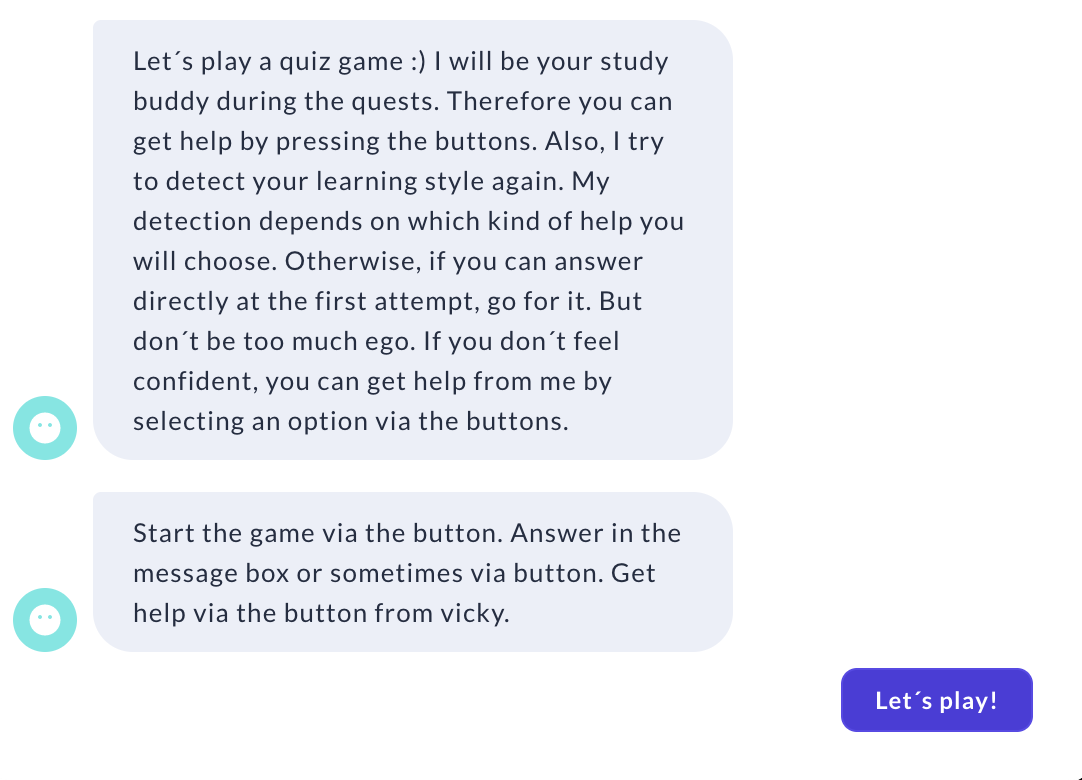
\includegraphics[width=0.65\linewidth]{images/VickyQuiz/gamestart.png}
  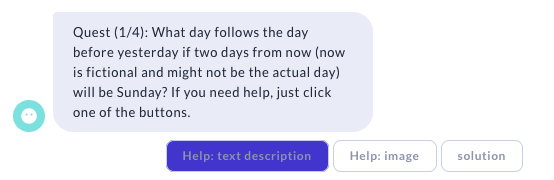
\includegraphics[width=0.65\linewidth]{images/VickyQuiz/Q0.png}
  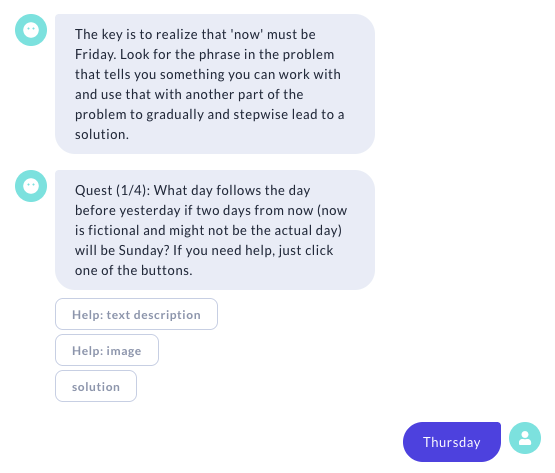
\includegraphics[width=0.65\linewidth]{images/Game/q1.1.png}
  \label{fig:Game_I}
\end{figure} 
\begin{figure}[H]
  \centering
  
\includegraphics[width=0.7\linewidth]{images/Game/q1.2.png}
  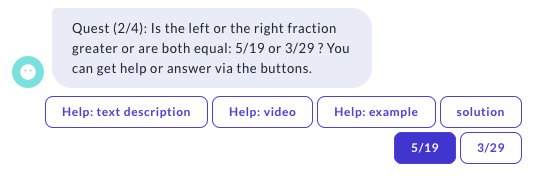
\includegraphics[width=0.7\linewidth]{images/VickyQuiz/Q1.png}
  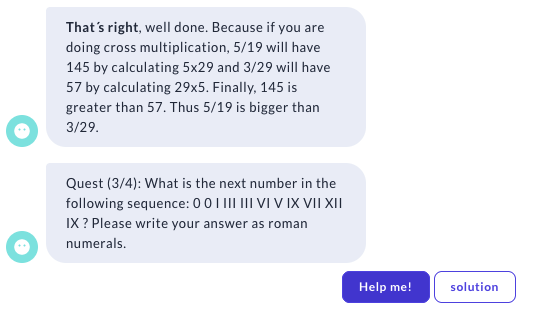
\includegraphics[width=0.7\linewidth]{images/VickyQuiz/Q2.png}
  \includegraphics[width=0.7\linewidth]{images/Game/Q3.33.png}

  \label{fig:Game_II}
\end{figure} 
\begin{figure}[H]
  \centering
  \includegraphics[width=0.7\linewidth]{images/Game/Q3.3.png}
  \includegraphics[width=0.7\linewidth]{images/VickyQuiz/Q4.png}
  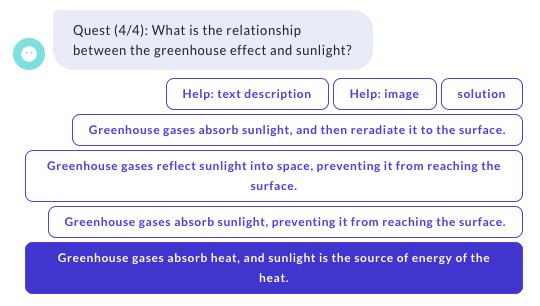
\includegraphics[width=0.7\linewidth]{images/VickyQuiz/Q5.png}
  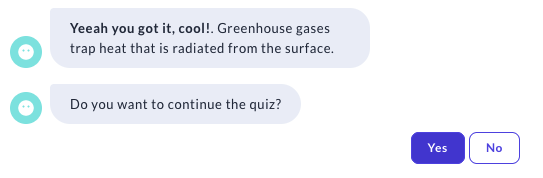
\includegraphics[width=0.7\linewidth]{images/VickyQuiz/Q6.png}
  \end{figure} 

\begin{figure}[H]
  \centering


  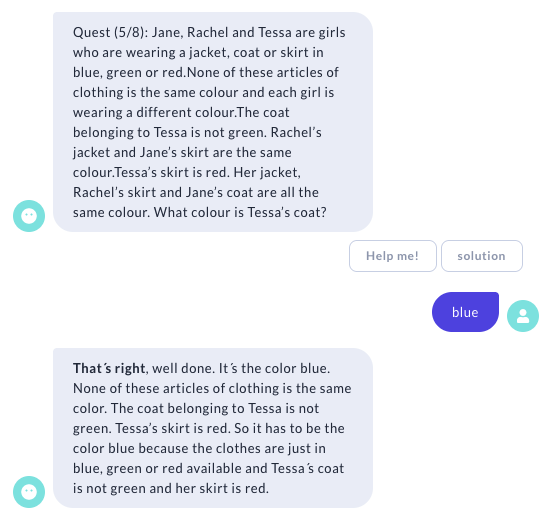
\includegraphics[width=0.7\linewidth]{images/VickyQuiz/Q7.png}
  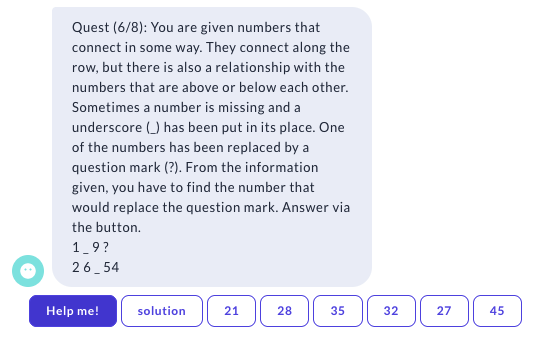
\includegraphics[width=0.7\linewidth]{images/VickyQuiz/Q8.png}
  
\includegraphics[width=0.7\linewidth]{images/VickyQuiz/Q8.1.png}

  \label{fig:Game_III}
\end{figure} 
\begin{figure}[H]
  \centering
  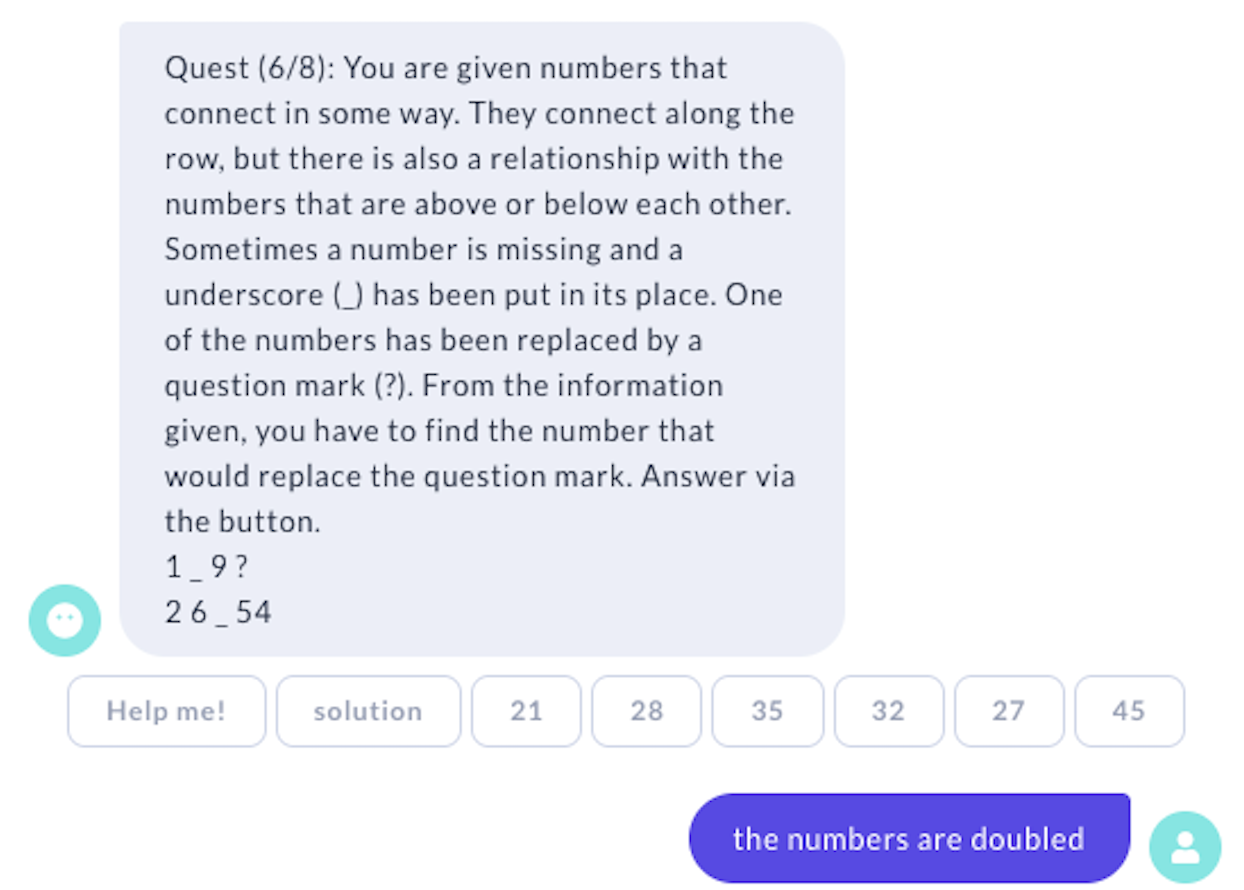
\includegraphics[width=0.7\linewidth]{images/VickyQuiz/Q9.1.png}
  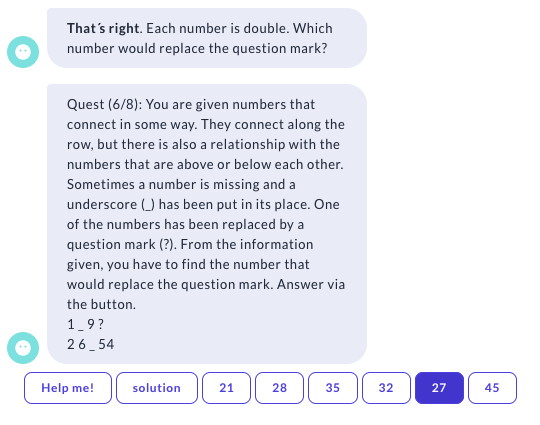
\includegraphics[width=0.7\linewidth]{images/VickyQuiz/Q10.png}
  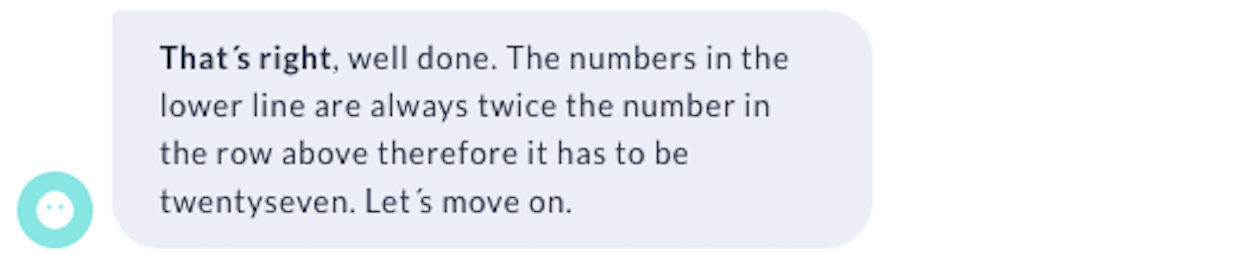
\includegraphics[width=0.7\linewidth]{images/VickyQuiz/Q11.1.png}

  \label{fig:Game_IV}
\end{figure} 
\begin{figure}[H]
  \centering
  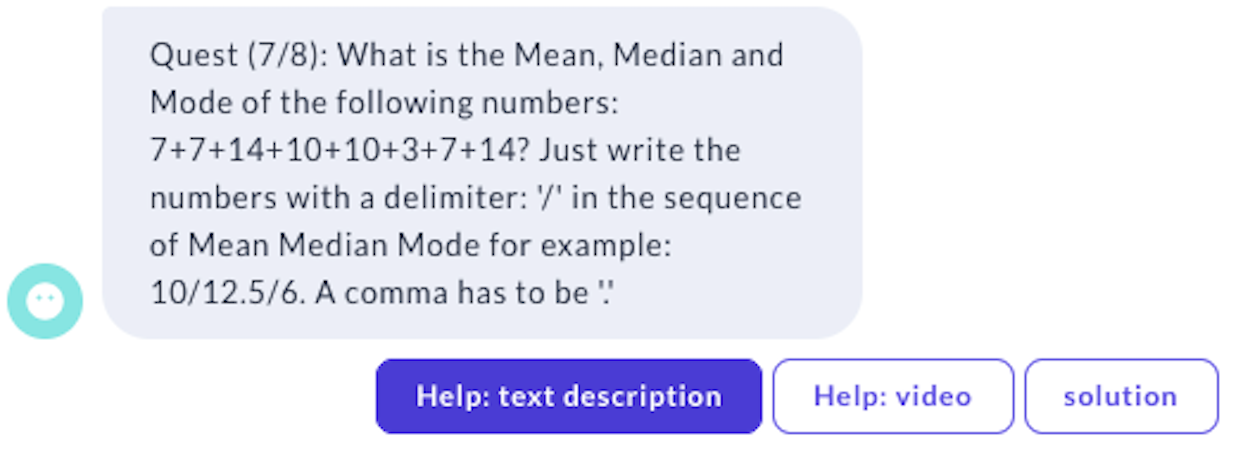
\includegraphics[width=0.7\linewidth]{images/VickyQuiz/Q11.2.png}
  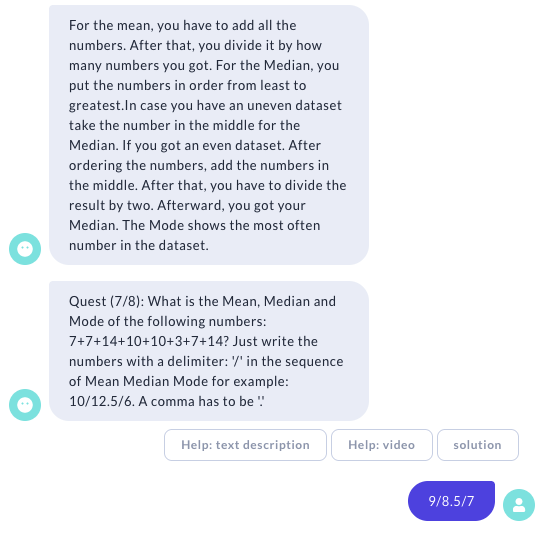
\includegraphics[width=0.7\linewidth]{images/VickyQuiz/Q13.png}
  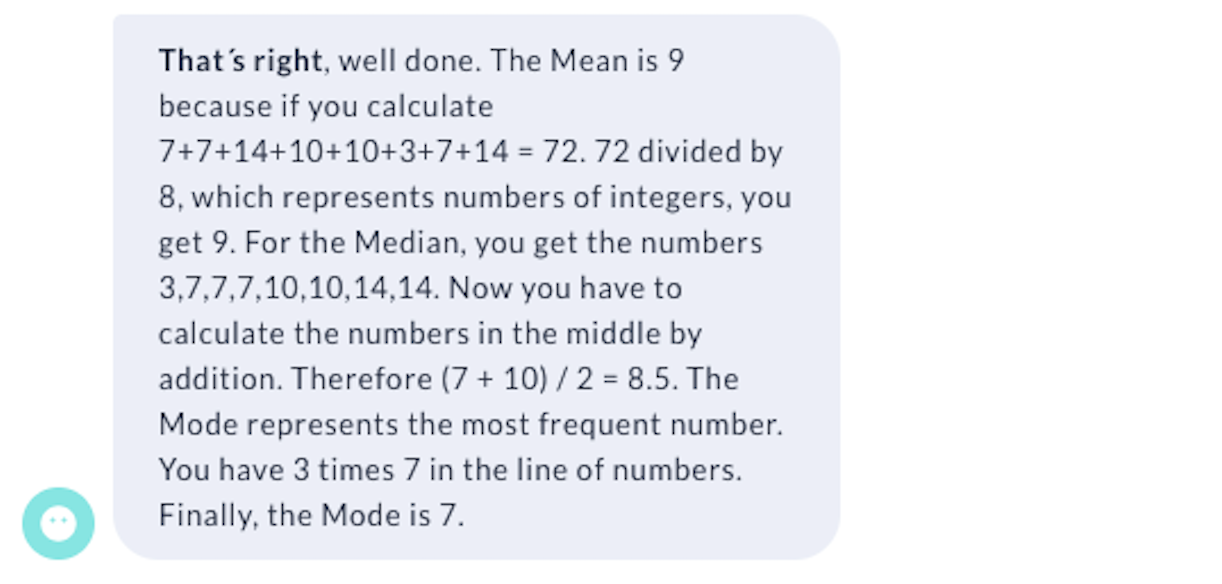
\includegraphics[width=0.7\linewidth]{images/VickyQuiz/Q12.1.png}
\end{figure} 
\begin{figure}[H]
  \centering

  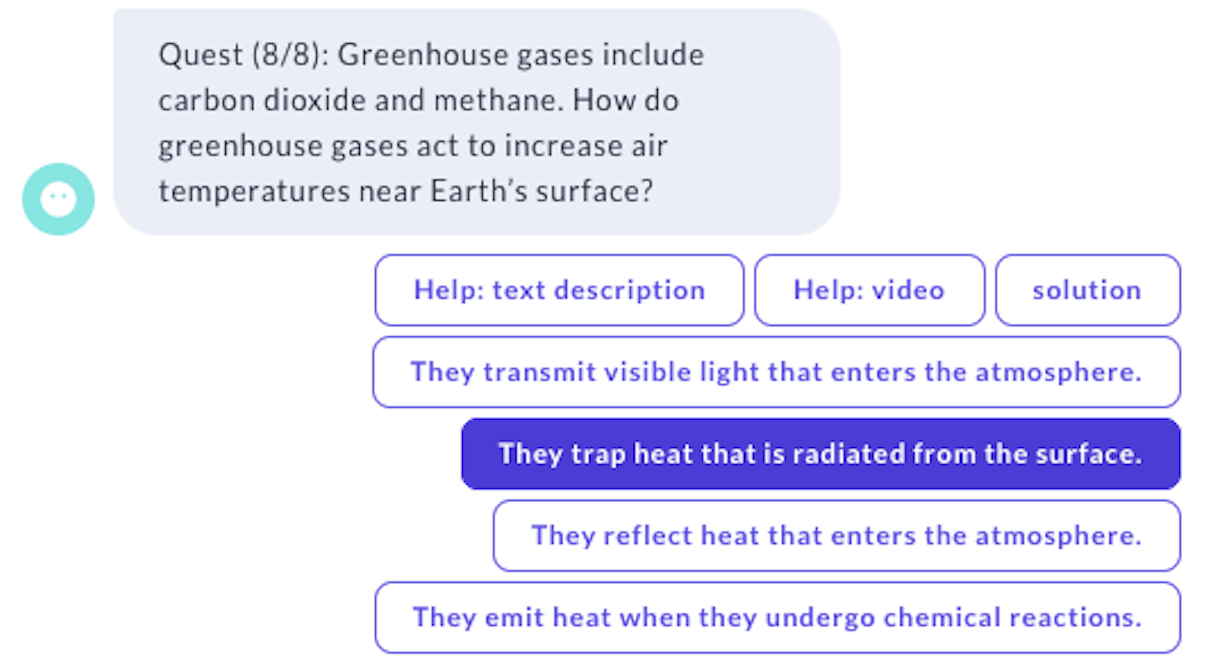
\includegraphics[width=0.7\linewidth]{images/VickyQuiz/Q12.2.png}
  
\includegraphics[width=0.7\linewidth]{images/VickyQuiz/Q13.5.png}
\label{fig:Anhang_Quiz-Spiel}
\end{figure} 

\chapter{Ressource: Erläuterung des Lernstils}   \label{tab:/Anhang_Erläuterung_des_Lernstils} 

\begingroup
  \footnotesize  
\begin{longtable}{|m{15cm}|}
  \hline \hline 
  \rowcolor[HTML]{EFEFEF}                                         
   
  \centering \arraybackslash \textbf{sensorischer Lerner}  \\ 
  \hline \hline 
  Sensorische Lerner können sich besser Fakten merken. 
  Sie lösen Probleme oft gerne mit bewährten Methoden und mögen 
  keine Komplikationen und Überraschungen. 
  Sie können sich Informationen am besten merken, wenn sie diese mit 
  der realen Welt in einen Zusammenhang bringen. Wenn Sie einen Kurs besuchen, 
  in dem der meiste Stoff  abstrakt und theoretisch ist, könnten Sie Schwierigkeiten haben.
  Also bitten Sie Ihren Tutor um konkrete Beispiele für die Konzepte und Verfahren und finden
  heraus, wie diese Konzepte in der Praxis angewendet werden. Wenn die Lehrkraft nicht 
  genügend konkrete Beispiele liefert, versuchen Sie, Beispiele in Ihrem Lehrbuch oder in 
  anderen Nachschlagewerken zu finden oder machen Sie ein Brainstorming mit Freunden
  oder Klassenkameraden.\\\hline 
  \hline  
  \rowcolor[HTML]{EFEFEF}                                         
   
  \centering \arraybackslash \textbf{intuitiver Lerner}  \\ 
  \hline \hline 
  Intuitve Lerner ziehen es oft vor, Möglichkeiten und Zusammenhänge zu entdecken.
  Sie neigen dazu, schnell und innovativ zu arbeiten.
  Wenn Sie sich in einem Kurs befinden, in dem es hauptsächlich um das Auswendiglernen
  und das Auswendiglernen von Formeln geht, kann Ihnen langweilig werden.
  Fragen Sie Ihren Tutor nach Interpretationen oder Theorien, welche die Fakten
  miteinander verbinden oder versuchen Sie, diese Zusammenhänge selbst zu finden.
  Möglicherweise neigen Sie bei Prüfungen auch zu Flüchtigkeitsfehlern, weil Sie
  ungeduldig sind und Wiederholungen nicht mögen (z. B. bei der Überprüfung Ihrer
  fertigen Lösungen). Nehmen Sie sich Zeit, die gesamte Frage zu lesen, bevor Sie mit
  der Beantwortung beginnen, und überprüfen Sie Ihre Ergebnisse.\\\hline 
  \hline     
  \rowcolor[HTML]{EFEFEF}                                         

  \centering \arraybackslash \textbf{visueller Lerner}  \\ 
  \hline \hline 
  Visuelle Lerner merken sich am besten, was sie sehen z. B. Bilder und Diagramme.
  Versuchen Sie eine visuelle Darstellung im Kursmaterial zu finden.
  Bereiten Sie eine Mind-Map vor, indem Sie die wichtigsten Punkte auflisten,
  diese in Kästchen oder Kreise einschließen und Linien mit Pfeilen zwischen den 
  Konzepten ziehen, um Verbindungen aufzuzeigen. Markieren Sie Ihre Notizen mit
  einem Textmarker, so dass alles, was mit einem Thema zu tun hat, die gleiche Farbe hat.\\\hline 
  \hline   
  \rowcolor[HTML]{EFEFEF}                                         
  
  \centering \arraybackslash \textbf{verbaler Lerner}  \\ 
  \hline \hline 
  Verbale Lerner können mit Worten mehr anfangen, z. B. mit schriftlichen und
  mündlichen Erklärungen. Schreiben Sie Zusammenfassungen oder Gliederungen
  des Lernstoffs in Ihren eigenen Worten. Die Arbeit in Gruppen kann besonders
  effektiv sein. Sie verstehen den Stoff besser, wenn Sie die Erklärungen Ihrer
  Mitschüler hören und Sie lernen noch mehr, wenn Sie selbst die Erklärungen geben. \\ \hline
  \hline     
  \rowcolor[HTML]{EFEFEF}                                         

  \centering \arraybackslash \textbf{aktiver Lerner}  \\ 
  \hline \hline 
  Aktive Lerner neigen dazu, Informationen am besten zu behalten und zu verstehen,
  wenn sie aktiv damit umgehen, z. B. indem sie diskutieren, anwenden oder anderen
  die Inhalte erläutern. Lernen Sie in einer Gruppe, in der die Mitglieder sich gegenseitig
  abwechselnd verschiedene Themen erklären. Arbeiten Sie mit anderen zusammen,
  um zu erraten, was Sie in der nächsten Prüfung gefragt werden, und überlegen Sie,
  wie Sie antworten werden. Sie werden Informationen immer besser behalten, wenn
  Sie Wege finden, etwas damit zu tun. \\ \hline
  \hline    
  \rowcolor[HTML]{EFEFEF}                                         
 
  \centering \arraybackslash \textbf{reflektiver Lerner}  \\ 
  \hline \hline 
  Reflektive Lerner denken lieber erst in Ruhe über Dinge nach.
  Wenn Sie im Unterricht keine Zeit zum Nachdenken über neue Informationen haben, 
  sollten Sie versuchen, diesen Mangel beim Lernen auszugleichen. Lesen Sie den Stoff
  nicht einfach nur ab oder lernen Sie ihn auswendig, halten Sie regelmäßig an, um das
  Gelesene zu überprüfen und über mögliche Fragen oder Anwendungen nachzudenken.
  Es kann hilfreich sein, kurze Zusammenfassungen des Gelesenen oder der
  Unterrichtsnotizen in eigenen Worten zu verfassen. Dies kann zusätzliche Zeit in
  Anspruch nehmen, aber es ermöglicht Ihnen, den Stoff besser zu behalten. \\ \hline
  \hline     
  \rowcolor[HTML]{EFEFEF}                                         

  \centering \arraybackslash \textbf{sequentieller Lerner}  \\ 
  \hline \hline 
  Sequentielle Lerner neigen dazu, sich den Stoff in linearen Schritten anzueignen,
  wobei jeder Schritt logisch auf den vorhergehenden folgt. Daher folgen Sie logischen,
  schrittweisen Wegen bei der Lösungsfindung. Nehmen  Sie sich die Zeit, den
  Vorlesungsstoff für sich selbst in logischer Reihenfolge zu  skizzieren. Auf lange Sicht
  werden Sie dadurch Zeit sparen. Sie können auch versuchen, Ihr globales Denken zu
  stärken, indem Sie jedes neue Thema, das Sie studieren, mit Dingen in Verbindung
  bringen, die Sie bereits kennen. Je mehr Sie dies tun, desto besser werden Sie das Thema verstehen. \\ \hline
  \hline   
  \rowcolor[HTML]{EFEFEF}                                         
  
  \centering \arraybackslash \textbf{globaler Lerner}  \\ 
  \hline \hline 
  Globale Lerner neigen dazu in großen Sprüngen zu lernen, indem sie Material fast
  wahllos aufnehmen, ohne Zusammenhänge zu erkennen und es dann plötzlich
  'kapieren'. Sie sind vielleicht in der Lage, komplexe Probleme schnell zu lösen
  oder Dinge auf neuartige Weise zusammenzufügen, sobald sie das große Ganze
  erfasst haben, aber sie haben vielleicht Schwierigkeiten zu erklären, wie sie das
  gemacht haben. Sie müssen erkennen, dass Sie erst das große Ganze eines Themas
  verstehen müssen, bevor Sie dieDetails beherrschen können. Wenn Ihr Tutor sich
  direkt in neue Themen stürzt, ohne sich die Mühe zu machen, zu erklären, wie Sie
  mit dem zurecht kommen, was Sie bereits wissen, kann das für Sie problematisch 
  werden. Glücklicherweise gibt es Schritte, die Sie unternehmen können, um das
  Gesamtbild schneller zu erfassen. Bevor Sie den ersten Abschnitt eines Kapitels
  in einem Kurs studieren, sollten Sie die gesamten Kurskapitel überfliegen, um sich
  einen Überblick zu verschaffen. Das mag anfangs zeitaufwändig sein, aber es
  erspart Ihnen später das ständige Wiederholen einzelner Teile. Anstatt sich jeden
  Abend kurz mit jedem Thema zu beschäftigen, ist es vielleicht produktiver,
  sich in großen Blöcken in einzelne Themen zu vertiefen. Versuchen Sie, das 
  Thema mit Dingen zu verknüpfen, die Sie bereits kennen. \\ \hline
  \caption[Lernstilerläuterung]{Lernstilerläuterung (eigene Darstellung, in Anlehnung an \parencite{FelderSoloman} } 

\end{longtable}
\endgroup  


\chapter{Umfrage} 
\section{Items: Wahrnehmung} \label{Umfrage}
\begingroup
\footnotesize 
\begin{longtable}{|m{6cm}|m{4cm}|m{5cm}|}
  \hline
    \rowcolor[HTML]{EFEFEF} 
    \centering \textbf{Item} &\centering \textbf{Item-Literatur} & \centering \arraybackslash  \textbf{Literaturnachweis} \\    \hline \hline
   Ich habe Vicky menschenähnlich wahrgenommen. & humanlike & \parencite[6 f.]{Holtgraves.2007}  \\ \hline
   Ich habe Vicky lebensecht wahrgenommen. & lifelike & \parencite[74]{Bartneck.2008} \parencite[5]{Powers.2006}  \\ \hline
   Ich habe Vicky natürlich wahrgenommen. & natural & \parencite[74]{Bartneck.2008} \parencite[5]{Powers.2006}  \\ \hline
   Ich fand Vickys Antworten elegant. & moving elegantly & \parencite[74]{Bartneck.2008}  \parencite[5]{Powers.2006}  \\ \hline
   Ich habe ein Gefühl des menschlichen Kontakts gespürt. & a sense of human contact  & \parencite[12]{Brendel.2021} \parencite[11]{Gefen.1997}  \\ \hline
   Ich habe ein Gefühl der menschlichen Wärme gespürt. & a sense of human warmth   & \parencite[12]{Brendel.2021} \parencite[11]{Gefen.1997}  \\ \hline
   Ich habe ein Gefühl der persönlichen Beziehung gespürt. & a sense of personalness   & \parencite[12]{Brendel.2021} \parencite[11]{Gefen.1997}  \\ \hline
   Ich habe ein Gefühl der Kontaktfreudigkeit gespürt. & a sense of sociability   & \parencite[12]{Brendel.2021} \parencite[11]{Gefen.1997}  \\ \hline
   Ich denke, Vicky interagiert wie eine Person. & a sense of human sensitivity   & \parencite[12]{Brendel.2021} \parencite[11]{Gefen.1997}  \\ \hline
    
   Ich kann Vicky vertrauen.& Trustworthiness  & \parencite[363]{Lee.2002} \\ \hline
  Ich denke, Vicky ist verlässlich. & reliability  & \parencite[153]{Jiang.2002} \\ \hline
  Ich denke, Vicky ist transparent. & /  & [*], [**]\footnote{* : eigenständig erstellt, wurde mit Reliabilitätsanalyse geprüft, **: wurde zusätzlich hinzugefügt, um zu prüfen, inwiefern der Lernende das Gefühl hatte, die bereitgestellten Informationen von Vicky rechtzeitig und ausreichend bekommen zu haben.  } \\ \hline

   Ich habe Vicky als unmenschlich wahrgenommen.& inhuman like   & \parencite[6 f.]{Holtgraves.2007}   \\ \hline
   Ich habe Vicky als seltsam wahrgenommen.& This character is strange.   & \parencite[13 ff.]{Tinwell.2014}    \\ \hline
   Ich habe Vicky als unsympathisch wahrgenommen.& /  & [*], [***]\footnote{*** : wurde zusätzlich hinzugefügt, um zu prüfen, inwiefern der Lernende das Gefühl hatte, Vicky als unheimlich wahrgenommen zu haben.}   \\ \hline
   Ich habe Vicky als unangenehm wahrgenommen.& /  & [*], [***]    \\ \hline

\end{longtable}
\label{tab:/Items_Wahrnehmung_Appendix} 
\endgroup

\section{Items: ARCS-Modell}\label{ARCSITEMS}
Im Folgenden sind die in der Umfrage verwendeten Items zum ARCS-Modell aufgelistet.\footnote{Items wurden eigenständig erstellt. Sie wurden mit der Reliabilitätsanalyse geprüft. } 

\begin{minipage}[t]{0.45\textwidth}
  \textbf{Attention}: fesselnd und anregend
  \begin{itemize}
      \item \glqq Vicky zu antworten hat mir Spaß gemacht.\grqq{} 
      \item \glqq Die Interaktion mit Vicky fiel mir leicht.\grqq{} 
      \item \glqq Ich könnte noch länger mit Vicky kommunizieren.\grqq{} 
  \end{itemize} 
  \end{minipage}
  \hfill
  \begin{minipage}[t]{0.45\textwidth}
  \textbf{Relevance}: nützlich und nachhaltig
  \begin{itemize}
  \item \glqq Ein CA könnte mir helfen öfter zu lernen.\grqq{}
  \item \glqq Ein CA könnte mir helfen frühzeitiger mit dem Lernen zu beginnen.\grqq{}
  \item \glqq Ein CA könnte mir beim Erkennen meiner eigenen Stärken und Schwächen helfen.\grqq{}\\
  \end{itemize}
  \end{minipage}
  
  \begin{minipage}[t]{0.45\textwidth}
  \textbf{Confidence}: unterstützend und begleitend
  \begin{itemize}
      \item \glqq Ein CA könnte mir bei meinem Lernerfolg helfen, welcher größtenteils auf meinen eigenen Bemühungen basiert.\grqq{}
      \item \glqq Ein CA könnte mir beim Setzen von Lernzielen helfen, welche ich durch meine eigenen Bemühungen erreiche.\grqq{} 
  \end{itemize}
  \end{minipage}
  \hfill
  \begin{minipage}[t]{0.45\textwidth}
  \textbf{Statisfaction}: zufriedenstellend und effektiv 
  \begin{itemize}
  \item \glqq Die Interaktion mit Vicky hat mich während des Quiz-Spiels motiviert.\grqq{} 
  \item \glqq Ein CA könnte mir bei der Aufrechterhaltung der Motivation helfen.\grqq{}  
  \item \glqq Ein CA könnte mir helfen im richtigen Tempo zu lernen.\grqq{}
  \end{itemize}
  \end{minipage}
  
  \begin{minipage}[t]{0.45\textwidth}
      \begin{itemize}
          \item \glqq Ein CA könnte mir bei der Strukturierung meines Lernens helfen.\grqq{}\\
      \end{itemize}
  \end{minipage}

  \section{Items: situativer Faktor} \label{SF}
  
  Die im folgenden genannten Items beziehen sich auf den situativen Faktor des Rahmenmodells von Rheinberg u.a. (2000)\footnote{Items wurden eigenständig erstellt. Sie wurden mit der Reliabilitätsanalyse geprüft. }: 
  \begin{itemize}
      \item \glqq Vicky ist ein virtueller Begleiter für mich geworden.\grqq{} 
      \item \glqq Ein CA könnte mir eine Art der sozialen Kontrolle bzgl. der Erreichung des Lernziels geben.\grqq{} 
      \item \glqq Ein CA könnte mir eine soziale Bindung geben.\grqq{} \\
  \end{itemize}
  

\section{Kommentare Teilbereich 2 \& 3} \label{tab:/Kommentare_Teilbereich_2} 

\begingroup
\footnotesize 
\begin{longtable}{|m{2cm}|m{13cm}|}
    \hline
    \rowcolor[HTML]{EFEFEF} 
    \centering \textbf{Index} &\centering \arraybackslash    \textbf{Kommentar} \\    \hline \hline
    \centering  \arraybackslash  1 &  Wie sicher bist du dir bei meinem Lernstil? \\ \hline
    \centering  \arraybackslash  2 &  Römische Zahlen    \\ \hline
    \centering  \arraybackslash  3 &  römische zahlen    \\ \hline
    \centering  \arraybackslash  4 &  ich bin nicht gut mit logischen Zahlen    \\ \hline
    \centering  \arraybackslash  5 &  Die Fragen waren überwiegend mathelastig    \\ \hline
    \centering  \arraybackslash  6 &  Mean Median and Mode, waren mir als Vokabeln nicht geläufig, das Video hat ausreichend erklärt    \\ \hline
    \centering  \arraybackslash  7 &  Es hat für mich keinen Unterschied gemacht wie ich antworten sollte     \\ \hline
    \centering  \arraybackslash  8 &  eigene Formulierungen fallen leichter um sich gezielt auszudrücken     \\ \hline
    \centering  \arraybackslash  9 &  Es ging schneller über die Buttons zu antworten.     \\ \hline
    \centering  \arraybackslash  10 &  Buttons: zeitsparend     \\ \hline
    \centering  \arraybackslash  11 &  Buttons sind praktischer, wenn man einer der Möglichkeiten zustimmt, aber mit Textfeldern kann man individueller antworten.     \\ \hline
    \centering  \arraybackslash  12 &  Habe beides verwendet    \\ \hline
    \centering  \arraybackslash  13 &  Buttons, da es schneller geht. Also sofern es nur vorgegebene Möglichkeiten gibt.   \\ \hline
    \centering  \arraybackslash  14 &  Es war eine leicht verständliche Kommunikation     \\ \hline
    \centering  \arraybackslash  15 &  Ja, beim Quiz. Vielleicht auch zu lange Fragen     \\ \hline
    \centering  \arraybackslash  16 &  Manchmal war ich davon frustriert, dass Vicky nur eine bestimmte Antwort erwartet. Man war gezwungen ein vorher vorgegebenen Stichpunkt als Antwort zu geben. Die Anwort war aus meiner Sicht nicht immer eindeutig. Habe mich dadurch teilweise missverstanden gefühlt    \\ \hline
    \centering  \arraybackslash  17 &  Eine sehr gute und realistische Einschätzung meines Lernstils    \\ \hline
    \centering  \arraybackslash  18 &  Ich denke mein Lernstil wurde überwiegend gut eingeschätzt und getroffen   \\ \hline

    
\end{longtable}
\endgroup


\section{Positive Aspekte über die Interaktion mit Vicky} \label{tab:/PostiveAspekte} 

\begingroup
\footnotesize 
\begin{longtable}{|m{2cm}|m{7cm}|m{6cm}|}
    \hline
    \rowcolor[HTML]{EFEFEF} 
    \centering \textbf{Index} &\centering   \textbf{Positiver Aspekt}&\centering \arraybackslash  \textbf{Kategorie}\\    \hline \hline
    \centering  \arraybackslash  1 & Schnelligkeit, Satzformulierung, Fragestellung  & schnell, verständlich   \\ \hline
    \centering  \arraybackslash  2 & Gute Einschätzung und passende Fragen zu den jeweiligen Antwortmöglichkeiten & verständlich     \\ \hline
    \centering  \arraybackslash  3  & Schnelle Antworten, Kennzeichnungen in Fett, Menschliche Umgangssprache & schnell, verständlich, authentisch    \\ \hline
    \centering  \arraybackslash  4 & straight forward, überwiegend klare Formulierungen, verständliche und kurz gehaltene Nachrichten & verständlich    \\ \hline
    \centering  \arraybackslash  5 & Einfach, leicht verständlich, hilsbereit & verständlich, hilsbereit \\ \hline
    \centering  \arraybackslash  6 & kurze knappe Fragen, authentisch & schnell, authentisch   \\ \hline
    \centering  \arraybackslash  7 & charmante Antworten & freundlich  \\ \hline
    \centering  \arraybackslash  8 & Spaß & Spaß  \\ \hline
    \centering  \arraybackslash  9 &  Sehr nett, verständlich, einfache Interaktion  & freundlich, verständlich  \\ \hline
    \centering  \arraybackslash  10 &   Hilfsbereit, schnell & hilsbereit, schnell \\\hline
    \centering  \arraybackslash  11 &  Freundliche Antworten, Übersichtliches User-Interface, nicht viel unnötige Beiträge & freundlich, verständlich \\ \hline
    \centering  \arraybackslash  12 & Man kann seinen Lernstil herausfinden inkl. Erklärungen, man kann smalltalk führen (menschlich), er kann Hilfestellungen geben & hilfsbereit, authentisch  \\ \hline
    \centering  \arraybackslash  13 & Vicky meldet Unklarheiten deutlich zurück, motiviert & authentisch, motivierend\\ \hline
    \centering  \arraybackslash  14 & Vicky ist sehr freundlich, Fragen und Aussagen leicht verständlich  & freundlich, verständlich\\ \hline
    \centering  \arraybackslash  15 & Er spricht einen persönlich an, er kann auch „Smalltalk“ führen, Er ist sympathisch. & authentisch \\ \hline
    \centering  \arraybackslash  16 & Nett, hilfsbereit, macht Spass & freundlich, hilfsbereit, Spaß\\ \hline
    \centering  \arraybackslash  17 & nettes Quiz, einfaches Englisch, unkomplizierter Umgang & Spaß, verständlich \\ \hline
    \centering  \arraybackslash  18 & Freundlich & freundlich\\ \hline
    \centering  \arraybackslash  19 & freundlich, hilfsbereit & freundlich, hilfsbereit\\ \hline
    \centering  \arraybackslash  20 & freundlich & freundlich \\ \hline
\end{longtable}
\endgroup


\section{Negative Aspekte über die Interaktion mit Vicky} \label{tab:/NegativeAspekte} 

\begingroup
\footnotesize 
\begin{longtable}{|m{2cm}|m{7cm}|m{6cm}|}
  \hline
    \rowcolor[HTML]{EFEFEF} 
    \centering \textbf{Index} &\centering \textbf{Negativer Aspekt} & \centering \arraybackslash  \textbf{Kategorie} \\    \hline \hline
    \centering  \arraybackslash  1 &  Antwort wurde nicht verstanden & unflexibel  \\ \hline
    \centering  \arraybackslash  2 &  Dadurch dass ich schon Chatbots geringfügig kannte, wusste, ich dass keine wirkliche Person auf der anderen Seite sitzt & unmenschlich  \\ \hline
    \centering  \arraybackslash  3 &  etwas unflexibel in der Antwortverarbeitung des Nutzers & unflexibel \\ \hline
    \centering  \arraybackslash  4 &  Unflexibel, an bestimmte Antworten gebunden & unflexibel \\ \hline
    \centering  \arraybackslash  5 &  auf Englisch & Englisch\\ \hline
    \centering  \arraybackslash  6 &  Bilder oder Videos im Chat wären schön anstatt auf den Link zu klicken, Erläuterung des Lernstil-Typs mit Video da der lange Text eher unattraktiv ist zu lesen, Quiz zu schwer hatte dann nicht so Lust nachzudenken & keine Verwendung von Videos/Bildern, zu schweres Quiz \\\hline
    \centering  \arraybackslash  7 &  Die Quizfragen waren zu lang, da habe ich weniger lust gehabt. Vielleicht kann man eher vorher fragen, was man machen möchte. Keine Bilder im Chat. Wenig emotionen. & zeitintensiv, keine Verwendung von Videos/Bildern, unmenschlich \\ \hline
    \centering  \arraybackslash  8 &  zu geringer Wortschatz, eingeschränktes Verständnis bei offenen Fragen & unflexibel \\ \hline
    \centering  \arraybackslash  9 &   es bleibt eine Maschine, hat noch ein paar Schwierigkeiten mit Formulierungen & unmenschlich, unflexibel \\ \hline
    \centering  \arraybackslash  10 &   Er versteht manchmal noch nicht alles, sein Antwortspektrum kann noch erweitert werden & unflexibel\\ \hline
    \centering  \arraybackslash  11 &   Koennte etwas freier in den antworten sein & unflexibel \\ \hline
    \centering  \arraybackslash  12 &   Es kostet einiges an Zeit & zeitintensiv\\ \hline
    \centering  \arraybackslash  13 &   Wenig emotionen &  unmenschlich\\ \hline
    \centering  \arraybackslash  14 &   mannchmal unflexibel was die Antwortmöglichkeit angeht & unflexibel\\ \hline
\end{longtable}
\endgroup

\pagebreak

\section{Vicky-Interaktion motivierend/ unmotivierend}\label{tab:/VIMUM} 

m: motivierend\\
um: unmotivierend 
\begingroup
\footnotesize 
\begin{longtable}{|m{2cm}|m{7cm}|m{6cm}|}
  \hline
    \rowcolor[HTML]{EFEFEF} 
    \centering \textbf{Index} &\centering \textbf{Aussage} & \centering \arraybackslash  \textbf{Kategorie} \\    \hline \hline
    \centering  \arraybackslash  1 & Die Antworten nach einer richtig gegebenen Antwort waren passend und haben mich motiviert & Spielerische Komponente (m)  \\ \hline
    \centering  \arraybackslash  2 & Per Quiz nicht so langweilig wie normales lernen& Spielerische Komponente (m)   \\ \hline
    \centering  \arraybackslash  3 & durch die direkten Fragen wurde man motiviert in entsprechender Güte zu antworten um den Gesprächspartner zufrieden zu stellen.& Dialog (m)   \\ \hline
    \centering  \arraybackslash  4 & Ich war motiviert die richtigen Antworten zu geben							 & Spielerische Komponente (m)   \\ \hline
    \centering  \arraybackslash  5 & Ich habe es eher als motivierend wahrgenommen. Der Austausch mit Vicky könnte das Lernen angenehmen und spannender machen. 							 &  Dialog (m)   \\ \hline
    \centering  \arraybackslash  6 &Vicky hat mich in dem Sinne motiviert (vor allem bei dem Quiz), am ball zu bleiben und es immer wieder zu versuchen
     wie beispielsweise durch die Tipps etc. Weiterhin positiv empfand ich, dass sie nicht gewertet hat, wenn etwas falsch war bzw. ob, etwas gut oder schlecht ist. 
      Außerdem wurde man gelobt, was ich auch als motivierend empfand. 							  & Spielerische Komponente (m)  \\ \hline
    \centering  \arraybackslash  7 & Die Hilfestellung hat mich unterstützt und weit genug in die richtige Richtung gewiesen als das ich dann die Lösung selber
     herausfinden konnte. Dadurch hatte ich einen Erfolg ohne das Gefühl bekommen zu haben, dass mir die Lösung vorgesagt wurde													 &  Spielerische Komponente (m)  \\ \hline
    \centering  \arraybackslash  8 & Das Gespräch war motivierend am Anfang, weil ich hier spontan ohne Nachzudenken   
    antworten konnte und Vicky automatisch daraus den Lernstil gemacht hat. Das Quiz war eher unmotivierend weil ich nachdenken musste und vieles nicht konnte. 							 &  Dialog (m), Spielerische Komponente (um) \\ \hline
    \centering  \arraybackslash  9 & Vicky benutzt positive Rückmeldung, so dass man ein Erfolgsgefühl vermittelt bekommt. 							 &  Spielerische Komponente (m)  \\ \hline
    \centering  \arraybackslash  10 & ein simples "wrong answer" war stellenweise ein wenig unmotivierend														 &  Spielerische Komponente (um) \\ \hline
    \centering  \arraybackslash  11 &Ein direkter Austausch während es Lernens ist hilfreich, da es eine gewisses Maß an Kontrolle generiert und daher hilft am Ball zu bleiben.							 							 &  Dialog (m) \\ \hline
    \centering  \arraybackslash  12 & Ich denke wenn man regelmäßig mit Vicky kommunzieren würde könnte er auf jeden Fall eine motivierende Rolle beim Lernen spielen.														 &  Dialog (m) \\ \hline
    \centering  \arraybackslash  13 & Quiz hat mich motiviert														 &  Spielerische Komponente (m) \\ \hline
    \centering  \arraybackslash  14 & ich empfand es eher als motivierend, weil es Erklärmöglichkeiten gab und man somit bei der Lösung unterstützt wurde.																											 & Spielerische Komponente (m)  \\ \hline
\end{longtable}
\endgroup


\section{Wahrnehmung eines virtuellen Begleiters}\label{tab:/VB} 


\begingroup
\footnotesize 
\begin{longtable}{|m{2cm}|m{7cm}|m{6cm}|}
  \hline
    \rowcolor[HTML]{EFEFEF} 
    \centering \textbf{Index} &\centering \textbf{Aussage} & \centering \arraybackslash  \textbf{Kategorie} \\    \hline \hline
    \centering  \arraybackslash  1 & Würde ich gut finden 									 & Gut \\ \hline
    \centering  \arraybackslash  2 & Ich fand es gut								& Gut \\ \hline
    \centering  \arraybackslash  3 & Gut & Gut\\ \hline
    \centering  \arraybackslash  4 & Könnte durchaus ein motivierender Faktor sein und helfen, mehr Struktur in das Lernen als Solches und das Aufteilen der Lerninhalte zu erlangen.
    Man könnte Lernerfolge zudem ggf. besser quantifizieren.									& Motivierend, Lernuntersützend\\ \hline
    \centering  \arraybackslash  5 & Es könnte hilfreich sein									 & Hilfreich\\ \hline
    \centering  \arraybackslash  6 & sehr fördernd und wenig störend 									 & Gut \\ \hline
    \centering  \arraybackslash  7 & Könnte die Art zu lernen erleichtern, 
    da Vicky wie eine Assistenz die Lerninhalte strukturiert und je nach Lernstand die passenden Übungen ausspielt.									 & Lernuntersützend\\ \hline
    \centering  \arraybackslash  8 & An sich glaube ich, dass es vor allem am Anfang (des Studiums) hilfreich sein kann,
     um beispielsweise eine Orientierung zu bekommen oder auch um generelle Fragen zu stellen.								 & Hilfreich \\ \hline
    \centering  \arraybackslash  9 & Sehr hilfreich und angenehm.									 & Hilfreich\\ \hline
    \centering  \arraybackslash  10 & Würde ich super finden									& Gut\\ \hline 
     \centering  \arraybackslash  11 &Es könnte sehr zur Motivation und einem größeren Lernerfolg beitragen, von einem Chatbot
     "begleitet" zu werden, wenn dieser mehr Funktionalitäten haben könnte, als Lernstile zu klassifizieren.									 & Motivierend\\ \hline
     \centering  \arraybackslash  12 & motivierend, nice									& Motivierend\\ \hline
    \centering  \arraybackslash  13 & Es könnte hilfreich sein, wenn der Chatbot das Lernen strukturiert,
     Vorschläge machen könnte, in welcher Reihenfolge man Aufgaben abarbeitet oder auch Tipps gibt, wo man 
     am besten Informationen über ein bestimmtes Thema herbekommen kann.
     Das könnte zum Beispiel ein passendes Lernvideo oder ein Artikel sein, der zu dem klassifizierten Lerntypen passt. 									& Lernuntersützend\\ \hline
     \centering  \arraybackslash  14 &Fände ich gut. Weitere Funktionalitäten wären: Zum Beispiel eine 
    Hilfe beim Zeitmanagement, Handlungsempfehlungen für die Lernstile also was ich dann mit der Info
     machen kann (welche Methoden, Tools gut für mich sind), mich verbinden mit Leuten die auch meine 
     Lernstile haben damit ich für mich passende Lerngruppen finde. ALso auch generell Verbindung zu 
     Mitstudierenden schaffen (wenn ich ein Gruppenlerner bin).									 & Lernuntersützend\\ \hline
    \centering  \arraybackslash  15 & Als eine mögliche, hilfreiche Unterstützung.									& Hilfreich\\ \hline
    \centering  \arraybackslash  16 & Ungewohnt.									& Ungewohnt \\ \hline
    \centering  \arraybackslash 17 & Es könnte eine Motivation darstellen und eine Art der sozialen Kontrolle ausüben, sodass es leichter fällt stetig zu lernen und dabei zu bleiben.									 & Motiverend, Lernuntersützend\\ \hline
    \centering  \arraybackslash  18 & 
    Ich fände es gut, wenn Vicky mir  nervige Aufgaben abnehmen könnte wie Lernplan zusammenstellen. 									& Hilfreich\\ \hline

\end{longtable}
\endgroup


